\documentclass[12pt]{article}
\usepackage[hyphens]{url}
\usepackage[margin=1in]{geometry}
\usepackage{amsmath,amsthm,amssymb}
\usepackage{appendix}
\usepackage[USenglish]{babel}
\usepackage{bbm}
\usepackage{bm}
\usepackage{mathrsfs}
\usepackage[ruled,vlined]{algorithm2e}
\usepackage{array}
\usepackage[style=ieee,backend=biber]{biblatex}
\usepackage{caption}
\usepackage[autostyle=true,english=american]{csquotes}
\usepackage[multiple]{footmisc}
\usepackage{graphicx}
\usepackage{listings}
\usepackage{multirow}
\usepackage{placeins}
\usepackage{color}
\usepackage{subcaption}
\usepackage{tikz}
\usetikzlibrary{arrows}
\usetikzlibrary{bayesnet}
%\usepackage{lmodern}
%\usepackage[utf8]{inputenc}
%\usepackage[scaled]{beramono}
%\usepackage[T1]{fontenc}
\usepackage{fontspec}
\setmainfont[Ligatures=TeX]{FreeSerif}
\setsansfont[Ligatures=TeX]{Cantarell}
\setmonofont[Scale=MatchLowercase]{Hack}

\addbibresource{bib.bib}
\newcommand\numberthis{\addtocounter{equation}{1}\tag{\theequation}}
\setcounter{secnumdepth}{5}

\definecolor{mygreen}{rgb}{0,0.6,0}
\definecolor{mygray}{rgb}{0.5,0.5,0.5}
\definecolor{mymauve}{rgb}{0.58,0,0.82}

\lstset{ %
  backgroundcolor=\color{white},   % choose the background color; you must add \usepackage{color} or \usepackage{xcolor}
  basicstyle=\fontsize{11}{11}\ttfamily,        % the size of the fonts that are used for the code
  breakatwhitespace=false,         % sets if automatic breaks should only happen at whitespace
  breaklines=true,                 % sets automatic line breaking
  captionpos=b,                    % sets the caption-position to bottom
  commentstyle=\color{mygreen},    % comment style
  deletekeywords={...},            % if you want to delete keywords from the given language
  escapeinside={\%*}{*)},          % if you want to add LaTeX within your code
  extendedchars=true,              % lets you use non-ASCII characters; for 8-bits encodings only, does not work with UTF-8
  frame=single,                    % adds a frame around the code
  keepspaces=true,                 % keeps spaces in text, useful for keeping indentation of code (possibly needs columns=flexible)
  keywordstyle=\color{blue},       % keyword style
  language=Octave,                 % the language of the code
  morekeywords={*,...},            % if you want to add more keywords to the set
  numbers=left,                    % where to put the line-numbers; possible values are (none, left, right)
  numbersep=5pt,                   % how far the line-numbers are from the code
  numberstyle=\tiny\color{mygray}, % the style that is used for the line-numbers
  rulecolor=\color{black},         % if not set, the frame-color may be changed on line-breaks within not-black text (e.g. comments (green here))
  showspaces=false,                % show spaces everywhere adding particular underscores; it overrides 'showstringspaces'
  showstringspaces=false,          % underline spaces within strings only
  showtabs=false,                  % show tabs within strings adding particular underscores
  stepnumber=2,                    % the step between two line-numbers. If it's 1, each line will be numbered
  stringstyle=\color{mymauve},     % string literal style
  tabsize=2,                       % sets default tabsize to 2 spaces
  title=\lstname                   % show the filename of files included with \lstinputlisting; also try caption instead of title
}
\allowdisplaybreaks

\sloppy
\title{Variational Faculty Evaluations}
\author{Nozomu Okuda}
\date{June 9, 2016}

\setcounter{secnumdepth}{5}
\makeatletter
\renewcommand{\labelitemii}{$\diamond$}
\renewcommand{\labelitemiii}{\scriptsize$\blacksquare$}
\renewcommand{\bottomfraction}{.7}
\renewcommand{\textfraction}{.15}
\makeatother

\newcommand{\KL}{\operatorname{KL}}
\newcommand{\E}{\operatorname{E}}

\tikzset{main node/.style={circle, draw}}
\tikzset{hyper node/.style={rectangle, draw}}
\begin{document}
\maketitle

\section{Introduction}

This document consists of my explanation for how mean-field variational
inference on the faculty evaluations model is derived.  Another tutorial
deriving essentially the same model can be found in \autocite{foxvartut} and in
\autocite{wikivar}.  This tutorial is different in that it derives the model
with respect to variance instead of with respect to precision (which is the way
the other two tutorials make their approach).

While I have written another variational inference tutorial \autocite{myvarlda},
I use a different approach here in deriving the update equations; in addition,
the previous tutorial considers the very different model of latent Dirichlet
allocation.\footnote{As it turns out, the approach I take for deriving the
update equations for this faculty evaluations model is the approach Kevin Black
takes in his variational tutorial for LDA \autocite{kb}.}

I assume that readers of this document are familiar with basic probability
theory, probabilistic graphical models, and mathematical notation.  It may also
be helpful to be familiar with Gibbs sampling.

The impetus for this formulation is as an exercise for a Bayesian statistics
class I am taking, taught by Dr. Kevin Seppi.  After presenting a previous
version of this document in class, the students pointed out errors.  Thanks to
them for helping me fix the document.

The source code for this document can be found at
\url{https://github.com/nOkuda/variationalnotes}, in the \texttt{varfac}
directory.  I use \texttt{xelatex} to produce this document.

This document was last updated on Jun 14, 2017, in order to fix a few mistakes.

\section{Variational Inference}

\subsection{Main Ideas}

Even if you do not understand anything else from this tutorial, at least keep
these points in mind:

\begin{itemize}
    \item Variational inference is a method (like Gibbs sampling) for
        approximating the joint distribution represented by a graphical model.
    \item Variational inference makes simplifying assumptions on the graphical
        model.
    \item Tuning the parameters on the simplified model can lead to a model
        close enough to the real model that we can use the simplified model
        instead.
    \item It takes multiple exposures to understand variational inference.
\end{itemize}

We begin our discussion by speaking in generalities.  We then apply the
principles we consider to the faculty evaluations model.

\subsection{Getting Close:  KL Divergence}

Suppose that we have two probability distributions, $r$ and $s$.  How might we
measure how similar the two are?

Conveniently, people have already thought long and hard about this question.
They suggest measuring the difference of $s$ from $r$ instead.  So the smaller
the difference, the more similar $s$ is to $r$.  This difference is called the
Kullback-Leibler Divergence (KL Divergence).\footnote{KL Divergence is not a
metric or distance, since the value from one distribution to another is not the
same value as the other to the one.} KL Divergence is defined:
\begin{align}\label{eq:kldivergence}
    \KL(r(x)\parallel s(x)) &\triangleq \int_{-\infty}^{\infty} r(x)
    \log{\frac{r(x)}{s(x)}}dx
    \nonumber \\
    &= \E_{r(x)}[\log \frac{r(x)}{s(x)}]
    \nonumber \\
    &= \E_{r(x)}[\log r(x)] - \E_{r(x)}[\log s(x)]
\end{align}
which we would read \enquote{the KL Divergence of $s$ from $r$}.

Intuitively, KL Divergence adds up how different $s(x)$ is from $r(x)$ at each
point along their domains.\footnote{There are some caveats to be aware of if you
intend to implement KL Divergence in code; you can find most of them in
\autocite{wikikl}.}  Fortuitously, the way to solve for this difference is the
difference of two expectations.\footnote{If you are familiar with information
theory, you might recognize that one of these terms is the negative of entropy.}

\subsection{Beginning the Derivation}

Now suppose that the model we are interested in is $p$.  As promised, we are
going to approximate it with a simpler model; let's call this simpler model $q$.
Let's call our data $D$ and our unknown random variables $\vec{x}$.  From a
machine learning standpoint, this means that we want to maximize $p(\vec{x}|D)$,
the probability of the settings of our random variables given the data.  It
turns out that maximizing $p(\vec{x}|D)$ is hard.

\subsection{Simplicity:  Mean Field Assumption}

So now you might ask how $q$ is simpler than $p$.  For this tutorial, we make
the mean field assumption for constructing our simplified model.\footnote{Why
what we're about to do is called the mean field assumption is not entirely clear
to me.}  The reason that $p$ is hard in general is that two (or more) unobserved
nodes point into the same observed node (see, for example,
Fig.~\ref{fig:pmodel}).  Thus, influence flows between these unobserved nodes.
The mean field assumption says that this influence is minimal.  Thus, $q$ is
like $p$ except that all arrows pointing into the observed node(s) are
erased.\footnote{In fact, $q$ doesn't even have nodes for $D$.}  Mathematically,
this means that $q$ is fully factorizable:
\begin{align}\label{eq:q}
    q(\vec{x}) &= \prod_{i=1}^{N} q(x_{i})
\end{align}
An example of a graphical model under the mean field assumption is in
Fig.~\ref{fig:qmodel}

\subsection{Continuing the Derivation}

Recall that what we want is for $q(\vec{x})$ to be as close as possible to
$p(\vec{x}|D)$.  So let's minimize
\begin{align}
    \KL(q(\vec{x})\parallel p(\vec{x}|D)).&
    \nonumber \\
    \intertext{In an ideal world, we would like}
    \KL(q(\vec{x})\parallel p(\vec{x}|D)) &= 0.
    \nonumber \\
    \intertext{But accepting reality, we can allow for some constant $C$ which will be the
    closest we can get $q(\vec{x})$ to $p(\vec{x}|D)$:}
    \KL(q(\vec{x})\parallel p(\vec{x}|D)) &= C.
\end{align}

Let's put in the definition of KL Divergence:
\begin{align}
    \E_{q(\vec{x})}[\log q(\vec{x})] - \E_{q(\vec{x})}[\log p(\vec{x}|D)] = C.
    \nonumber
\end{align}

And now, we do algebra.
\begin{align}
    \E_{q(\vec{x})}[\log q(\vec{x})] &= C + \E_{q(\vec{x})}[\log p(\vec{x}|D)]
    \nonumber \\
    \intertext{Apply the mean field assumption:}
    \E_{q(\vec{x})}[\log \prod_{i} q(x_i)] &= C + \E_{q(\vec{x})}[\log p(\vec{x}|D)]
    \nonumber \\
    \intertext{Log of product is sum of logs:}
    \E_{q(\vec{x})}[\sum_{i}\log q(x_i)] &= C + \E_{q(\vec{x})}[\log p(\vec{x}|D)]
    \nonumber \\
    \intertext{Expectation of sum is sum of expectations:}
    \sum_{i}\E_{q(\vec{x})}[\log q(x_i)] &= C + \E_{q(\vec{x})}[\log p(\vec{x}|D)]
    \nonumber \\
    \intertext{Irrelevant terms in expectation fall out (if this is not obvious,
    think about the definition of expectations and the mean field assumption):}
    \sum_{i}\E_{q(x_i)}[\log q(x_i)] &= C + \E_{q(\vec{x})}[\log p(\vec{x}|D)]
    \nonumber \\
    \intertext{Separate $x_k$ out from the rest:}
    \E_{q(x_k)}[\log q(x_k)] + \sum_{i \neq k}\E_{q(x_i)}[\log q(x_i)] &=
    C + \E_{q(x_k)}[\E_{q(\vec{x}_{\neg k})}[\log p(\vec{x}|D)]]
    \nonumber \\
    \intertext{Gather terms constant with respect to $x_k$ into $C_{\neg k}$:}
    \E_{q(x_k)}[\log q(x_k)] &=
    C_{\neg k} + \E_{q(x_k)}[\E_{q(\vec{x}_{\neg k})}[\log p(\vec{x}|D)]]
    \nonumber \\
    \intertext{Apply definition of expectations:}
    \int q(x_k)\log q(x_k)dx_{k} &=
    C_{\neg k} + \int q(x_k)\E_{q(\vec{x}_{\neg k})}[\log p(\vec{x}|D)]dx_{k}
    \nonumber \\
    \intertext{Take derivative of both sides with respect to $x_k$ (remember
    that if $F = \int f(x) dx, \frac{dF}{dx} = f(x)$):}
    q(x_k)\log q(x_k) &=
    q(x_k)\E_{q(\vec{x}_{\neg k})}[\log p(\vec{x}|D)]
    \nonumber \\
    \intertext{Divide both sides by $q(x_k)$:}
    \log q(x_k) &=
    \E_{q(\vec{x}_{\neg k})}[\log p(\vec{x}|D)]
    \nonumber \\
    \intertext{Exponentiate both sides:}
    q(x_k) &=
    \exp (\E_{q(\vec{x}_{\neg k})}[\log p(\vec{x}|D)])
\end{align}

We now have some guidance as to what $q(x_k)$ ought to look like.
Unfortunately, as we noted earlier, we can't calculate $p(\vec{x}|D)$ very
easily (that's why we went to the trouble of making up $q(\vec{x})$).  We do,
however, know how to calculate $p(x_k|\vec{x}_{\neg k}, D)$, assuming that
$\vec{x}_{\neg k}$ is held constant.  This assumption would be true within a
given iteration if we iteratively solve for $q(x_k)$ holding $\vec{x}_{\neg k}$
constant; at each iteration, we change $k$.  Let's try it out.
\begin{align}
    q(x_k) &=
    \exp (\E_{q(\vec{x}_{\neg k})}[\log p(\vec{x}|D)])
    \nonumber \\
    \intertext{Separate $x_{k}$ from the rest:}
    &=
    \exp (\E_{q(\vec{x}_{\neg k})}[\log p(x_k, \vec{x}_{\neg k}|D)])
    \nonumber \\
    \intertext{Apply definition of conditional probability:}
    &=
    \exp (\E_{q(\vec{x}_{\neg k})}[\log \frac{p(x_k, \vec{x}_{\neg k},D)}{p(D)}])
    \nonumber \\
    \intertext{Log of quotient is difference of logs:}
    &=
    \exp (\E_{q(\vec{x}_{\neg k})}[\log p(x_k, \vec{x}_{\neg k},D) - \log p(D)])
    \nonumber \\
    \intertext{Expectation of difference is difference of expectations:}
    &=
    \exp (\E_{q(\vec{x}_{\neg k})}[\log p(x_k, \vec{x}_{\neg k},D)] - \E_{q(\vec{x}_{\neg k})}[\log p(D)])
    \nonumber \\
    \intertext{Apply exponent rules:}
    &=
    \exp (\E_{q(\vec{x}_{\neg k})}[\log p(x_k, \vec{x}_{\neg k},D)]) \exp(- \E_{q(\vec{x}_{\neg k})}[\log p(D)])
    \nonumber \\
    \intertext{Note that $\exp(- \E_{q(\vec{x}_{\neg k})}[\log p(D)])$ is
    constant (because $D$ is constant):}
    &\propto
    \exp (\E_{q(\vec{x}_{\neg k})}[\log p(x_k, \vec{x}_{\neg k},D)])
    \label{eq:qformjoint}\\
    \intertext{Multiply by a constant (we still keep proportionality, since
    $\vec{x}_{\neg k}$ is constant, as is $D$):}
    &\propto
    \exp (\E_{q(\vec{x}_{\neg k})}[\log p(x_k, \vec{x}_{\neg k},D)])
    \exp (-\E_{q(\vec{x}_{\neg k})}[\log p(\vec{x}_{\neg k},D)])
    \nonumber \\
    \intertext{Apply exponent rules:}
    &=
    \exp (\E_{q(\vec{x}_{\neg k})}[\log p(x_k, \vec{x}_{\neg k},D)]
    -\E_{q(\vec{x}_{\neg k})}[\log p(\vec{x}_{\neg k},D)])
    \nonumber \\
    \intertext{Difference of expectations is expectation of difference:}
    &=
    \exp (\E_{q(\vec{x}_{\neg k})}[\log p(x_k, \vec{x}_{\neg k},D)
    -\log p(\vec{x}_{\neg k},D)])
    \nonumber \\
    \intertext{Difference of logs is log of quotient:}
    &=
    \exp (\E_{q(\vec{x}_{\neg k})}[\log \frac{p(x_k, \vec{x}_{\neg k},D)}
    {p(\vec{x}_{\neg k},D)}])
    \nonumber \\
    \intertext{Apply definition of conditional probability:}
    &=
    \exp (\E_{q(\vec{x}_{\neg k})}[\log p(x_k|\vec{x}_{\neg k},D)])
    \label{eq:qformcond}
\end{align}

So to summarize,
\begin{align}\label{eq:qform}
    q(x_k) &\propto
    \exp (\E_{q(\vec{x}_{\neg k})}[\log p(x_k, \vec{x}_{\neg k},D)])
    \nonumber \\
    &\propto
    \exp (\E_{q(\vec{x}_{\neg k})}[\log p(x_k|\vec{x}_{\neg k},D)])
\end{align}
Either form for $q(x_k)$ can work, so we should choose the easier one to work
for the given problem.\footnote{Blei \autocite{bleinotesvar} derives these forms
for $q(x_k)$ by differentiating the lower bound with respect to $q(x_k)$.  I
couldn't figure out how to do that, so I came up with this approach after
looking at Ormerod and Wand's attempt to explain the derivation
\autocite{ormerod2010explaining} (they likewise choose not to take Blei's
approach).}

You may be suspicious that we can find the joint $p(x_k, \vec{x}_{\neg k}, D)$
(or the conditional $p(x_k|\vec{x}_{\neg k}, D)$) when we've already said that
we can't find $p(\vec{x}|D)$.  To assuage your suspicions (at least in the case
of the joint), let's apply the principles we've just derived to an example.

\section{Faculty Evaluations Model}

We define the faculty evaluations model as
\begin{equation}
    \mu \mid \mu', \delta' \sim \text{Normal}(\mu', \delta')
\end{equation}
\begin{equation}
    \delta \mid \alpha, \beta \sim \text{InverseGamma}(\alpha, \beta)
\end{equation}
\begin{equation}
    y_{k} \mid \mu, \delta \sim \text{Normal}(\mu, \delta)
\end{equation}
where $y_{k}$ is an observed score, $\mu$ is the mean of the distribution which
generates the scores, and $\delta$ is the variance.  Note that the Normal
distribution is parameterized by mean and variance; the Inverse Gamma
distribution is parameterized by $\alpha$ and $\beta$.

The graphical model is shown in Fig.~\ref{fig:pmodel}.

\begin{figure}[h]
    \centering
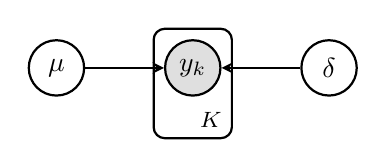
\begin{tikzpicture}[->, >=stealth, thick, scale=3.0]

    % Nodes

    \node[obs]                   (y)      {$y_{k}$} ; %
    \node[latent, left=of y]    (mu)      {$\mu$} ; %
    \node[latent, right=of y]    (delta)  {$\delta$}; %

    \edge {mu} {y}
    \edge {delta} {y}

    \plate {plate1} { %
        (y)
    } {$K$}; %

\end{tikzpicture}
    \caption{The true model of interest.  Note how $\mu$ and $\delta$ are
    pointing into the same observed nodes, thus making it difficult to infer
    $\mu$ and $\delta$.}
    \label{fig:pmodel}
\end{figure}

Since we have the evaluation data already, we are interested in the posterior
distributions of $\mu$ and $\delta$.

We know how to factor the joint probability of the model:
\begin{equation}
    p(\vec{x}, D) = p(\mu|\mu', \delta')p(\delta|\alpha, \beta)\prod_{k=1}^{K}p(y_{k}|\mu, \delta)
\end{equation}

So
\begin{align}
    \log{p(\vec{x}, D)} &= \log{p(\mu|\mu', \delta')} + \log{p(\delta|\alpha,
    \beta)} + \sum_{k=1}^{K}
    \log{p(y_{k}|\mu, \delta)} \nonumber \\
    &=
    \log{\left(\frac{1}{\sqrt{2\delta'\pi}}\exp{\left(-\frac{(\mu-\mu')^{2}}{2\delta'}\right)}\right)} +
    \log{\left(\frac{\beta^{\alpha}}{\Gamma(\alpha)}\delta^{-\alpha-1}\exp{\left(\frac{-\beta}{\delta}\right)}\right)}
    \nonumber \\
    &\quad\quad\quad\quad+ \sum_{k=1}^{K}
    \log{\left(\frac{1}{\sqrt{2\delta\pi}}\exp{\left(-\frac{(y_{k}-\mu)^{2}}{2\delta}\right)}\right)}
    \nonumber \\
    &= -\frac{1}{2} \log{(2\delta'\pi)} - \frac{(\mu - \mu')^{2}}{2\delta'} +
    \alpha \log{(\beta)} - \log{(\Gamma(\alpha))} - (\alpha + 1) \log{(\delta)}
    + \frac{-\beta}{\delta}\nonumber \\
    &\quad\quad\quad\quad+ \sum_{k=1}^{K} \left[-\frac{1}{2}
    \log{(2\delta\pi)} - \frac{(y_{k} - \mu)^{2}}{2\delta}\right] \nonumber \\
    &= -\frac{(\mu-\mu')^{2}}{2\delta'} - (\alpha+1)\log{(\delta)} +
    \frac{-\beta}{\delta} - \frac{K}{2}\log{(\delta)} -
    \frac{1}{2\delta}\sum_{k=1}^{K} (y_{k}-\mu)^{2} + C_p
    \label{eq:logp}
\end{align}
where $C_p$ is a constant holding the values not dependent on $\mu$ or $\delta$
in $p$.

\section{Deriving the Approximate Distribution}

Again, $q$ is our simplified model.  Because we made the mean field assumption,
the graphical model of $q$ looks like Fig.~\ref{fig:qmodel}.

\begin{figure}[h]
    \centering
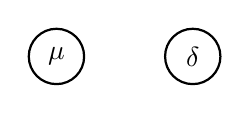
\begin{tikzpicture}[->, >=stealth, thick, scale=3.0]

    % Nodes

    \node[latent]    (mu)      {$\mu$} ; %
    \node[latent, right=of mu]    (delta)  {$\delta$}; %

\end{tikzpicture}
    \caption{The approximate model.  Note that in comparison to
    Fig.~\ref{fig:pmodel}, no observed nodes are present, and all of the
    connections to the observed nodes are gone.}
    \label{fig:qmodel}
\end{figure}

Let's start with $\mu$:
\begin{align}
    \intertext{Recall from Eq.~\ref{eq:qform} the form of $q(\mu)$:}
    q(\mu) &\propto \exp{(\E_{\neg q(\mu)}[\log{p(\mu, \delta, y_{1:K})}])}
    \nonumber \\
    &= \exp{(\E_{\neg q(\mu)}[\log{p(\vec{x}, D)}])}
    \nonumber \\
    \intertext{Apply Eq.~\ref{eq:logp}:}
    &= \exp{(\E_{\neg q(\mu)}[-\frac{(\mu-\mu')^2}{2\delta'}
    - (\alpha+1)\log{(\delta)} - \frac{\beta}{\delta}
    - \frac{K}{2}\log{(\delta)}
    - \frac{1}{2\delta} \sum_{k=1}^{K} (y_{k} - \mu)^2
    + C_p])}
    \nonumber \\
    &= \exp{}(-\E_{\neg q(\mu)}[\frac{(\mu-\mu')^2}{2\delta'}]
    - \E_{\neg q(\mu)}[(\alpha+1)\log{(\delta)}] - \E_{\neg
    q(\mu)}[\frac{\beta}{\delta}]
    - \E_{\neg q(\mu)}[\frac{K}{2}\log{(\delta)}]
    \nonumber \\
    &\qquad
    - \E_{\neg q(\mu)}[\frac{1}{2\delta} \sum_{k=1}^{K} (y_{k} - \mu)^2]
    + \E_{\neg q(\mu)}[C_p])
    \nonumber \\
    &= \exp{}(-\frac{(\mu-\mu')^2}{2\delta'}
    - \E_{\neg q(\mu)}[(\alpha+1)\log{(\delta)}] - \E_{\neg
    q(\mu)}[\frac{\beta}{\delta}]
    - \E_{\neg q(\mu)}[\frac{K}{2}\log{(\delta)}]
    \nonumber \\
    &\qquad
    - \E_{\neg q(\mu)}[\frac{1}{2\delta} \sum_{k=1}^{K} (y_{k} - \mu)^2]
    + C_p)
    \nonumber \\
    \intertext{Anything constant with respect to $\mu$ will be a constant we can
    ignore in the constant of proportionality:}
    &\propto \exp{(-\frac{(\mu-\mu')^2}{2\delta'}
    - \E_{\neg q(\mu)}[\frac{1}{2\delta} \sum_{k=1}^{K} (y_{k} - \mu)^2])}
    \nonumber \\
    &= \exp{(-\frac{(\mu-\mu')^2}{2\delta'}
        - \frac{\sum_{k=1}^{K}(y_{k}-\mu)^2}{2}\E_{\neg q(\mu)}[\frac{1}{\delta}]
    )}
    \nonumber \\
    &= \exp{(-\frac{\mu^2 - 2\mu\mu' +\mu'^2}{2\delta'}
        - \frac{\sum_{k=1}^{K}(y_{k}^2 -2y_{k}\mu + \mu^2)}{2}\E_{\neg q(\mu)}[\frac{1}{\delta}]
    )}
    \nonumber \\
    &= \exp{(-\frac{\mu^2 - 2\mu\mu' +\mu'^2}{2\delta'}
        - \frac{\sum_{k=1}^{K}y_{k}^2 -\sum_{k=1}^{K}2y_{k}\mu + \sum_{k=1}^{K}\mu^2}{2}\E_{\neg q(\mu)}[\frac{1}{\delta}]
    )}
    \nonumber \\
    &\propto \exp{(-\frac{\mu^2 - 2\mu\mu'}{2\delta'}
        - \frac{-\sum_{k=1}^{K}2y_{k}\mu + K\mu^2}{2}\E_{\neg q(\mu)}[\frac{1}{\delta}]
    )}
    \nonumber \\
    &= \exp{(-\frac{1}{2\delta'}\mu^2 + \frac{\mu'}{\delta'}\mu
        + (\sum_{k=1}^{K}y_{k}\mu - \frac{K}{2}\mu^2)\E_{\neg q(\mu)}[\frac{1}{\delta}]
    )}
    \nonumber \\
    &= \exp{(-\frac{1}{2\delta'}\mu^2 + \frac{\mu'}{\delta'}\mu
        + (\frac{\sum_{k=1}^{K}y_{k}\delta'}{\delta'}\mu
        - \frac{K\delta'}{2\delta'}\mu^2)\E_{\neg q(\mu)}[\frac{1}{\delta}]
    )}
    \nonumber \\
    &= \exp{(-\frac{1+K\delta'\E_{\neg q(\mu)}[\frac{1}{\delta}]}{2\delta'}\mu^2
    + \frac{\mu' + \E_{\neg q(\mu)}[\frac{1}{\delta}]\delta'\sum_{k=1}^{K}y_{k}}{\delta'}\mu
    )}
    \nonumber \\
    &= \exp{(-(\frac{1+\E_{\neg q(\mu)}[\frac{1}{\delta}]\delta'K}{2\delta'}\mu^2
    - \frac{\mu' + \E_{\neg q(\mu)}[\frac{1}{\delta}]\delta'\sum_{k=1}^{K}y_{k}}{\delta'}\mu
    ))}
    \nonumber \\
    \intertext{Complete the square and let the constant of proportionality take
    the constant:}
    &\propto
    \exp{(-\frac{1+\E_{\neg q(\mu)}[\frac{1}{\delta}]\delta'K}{2\delta'}
    (\mu
    - \frac{
    \mu' + \E_{\neg q(\mu)}[\frac{1}{\delta}]\delta'\sum_{k=1}^{K}y_{k}}
    {1 + \E_{\neg q(\mu)}[\frac{1}{\delta}]\delta'K})^2
    )}
\end{align}
Since $q(\mu)$ is a pdf, and since we know that it is proportional to the kernel
of a Normal distribution, we can see that
\begin{align}\label{eq:qmu}
    q(\mu) = N\left(\frac{\mu' + \E_{\neg q(\mu)}[\frac{1}{\delta}] \delta' \sum_{k=1}^{K}
    y_{k}}{1 + \E_{\neg q(\mu)}[\frac{1}{\delta}]\delta'K}, \frac{\delta'}{1 + \E_{\neg
    q(\mu)}[\frac{1}{\delta}]\delta'K}\right).
\end{align}

Now we need $q(\delta)$:
\begin{align}
    \intertext{Recall from Eq.~\ref{eq:qform} the form of $q(\delta)$:}
    q(\delta) &\propto \exp{(\E_{\neg q(\delta)}[\log p(\delta, \mu, y_{1:K})])}
    \nonumber \\
    &= \exp{(\E_{\neg q(\delta)}[\log p(\vec{x}, D)])}
    \nonumber \\
    \intertext{Apply Eq.~\ref{eq:logp}:}
    &= \exp{(\E_{\neg q(\delta)}[-\frac{(\mu-\mu')^2}{2\delta'}
    - (\alpha+1)\log{(\delta)} - \frac{\beta}{\delta}
    - \frac{K}{2}\log{(\delta)}
    - \frac{1}{2\delta} \sum_{k=1}^{K} (y_{k} - \mu)^2
    + C_p])}
    \nonumber \\
    &= \exp{}(-\E_{\neg q(\delta)}[\frac{(\mu-\mu')^2}{2\delta'}]
    - \E_{\neg q(\delta)}[(\alpha+1)\log{(\delta)}] - \E_{\neg
    q(\delta)}[\frac{\beta}{\delta}]
    - \E_{\neg q(\delta)}[\frac{K}{2}\log{(\delta)}]
    \nonumber \\
    &\qquad
    - \E_{\neg q(\delta)}[\frac{1}{2\delta} \sum_{k=1}^{K} (y_{k} - \mu)^2]
    + \E_{\neg q(\delta)}[C_p])
    \nonumber \\
    &= \exp{}(-\E_{\neg q(\delta)}[\frac{(\mu-\mu')^2}{2\delta'}]
    - (\alpha+1)\log{(\delta)} - \frac{\beta}{\delta}
    \nonumber \\
    &\qquad
    - \frac{K}{2}\log{(\delta)}
    - \E_{\neg q(\delta)}[\frac{1}{2\delta} \sum_{k=1}^{K} (y_{k} - \mu)^2]
    + C_p)
    \nonumber \\
    \intertext{Anything constant with respect to $\delta$ will be a constant we can
    ignore in the constant of proportionality:}
    &\propto \exp{(
    - (\alpha+1)\log{(\delta)} - \frac{\beta}{\delta}
    - \frac{K}{2}\log{(\delta)}
    - \E_{\neg q(\delta)}[\frac{1}{2\delta} \sum_{k=1}^{K} (y_{k} - \mu)^2
    ])}
    \nonumber \\
    &= \exp{(
    - (\alpha+1)\log{(\delta)} - \frac{\beta}{\delta}
    - \frac{K}{2}\log{(\delta)}
    - \frac{1}{2\delta} \E_{\neg q(\delta)}[\sum_{k=1}^{K} (y_{k} - \mu)^2
    ])}
    \nonumber \\
    &= \delta^{-(\alpha+\frac{K}{2}) - 1}\exp{(
    \frac{-\beta}{\delta}
    - \frac{1}{2\delta} \E_{\neg q(\delta)}[\sum_{k=1}^{K} (y_{k} - \mu)^2
    ])}
    \nonumber \\
    &= \delta^{-(\alpha+\frac{K}{2}) - 1}\exp{(
    \frac{-2\beta}{2\delta}
    - \frac{1}{2\delta} \E_{\neg q(\delta)}[\sum_{k=1}^{K} (y_{k}^2 -2y_{k}\mu +
    \mu^2)
    ])}
    \nonumber \\
    &= \delta^{-(\alpha+\frac{K}{2}) - 1}\exp{(
    \frac{-2\beta
    - \E_{\neg q(\delta)}[\sum_{k=1}^{K} (y_{k}^2 -2y_{k}\mu +
    \mu^2)]}{2\delta}
    )}
    \nonumber \\
    &= \delta^{-(\alpha+\frac{K}{2}) - 1}\exp{(
    \frac{-2\beta
    - \sum_{k=1}^{K} y_{k}^2 + \sum_{k=1}^{K}2y_{k}
    \E_{\neg q(\delta)}[\mu] - K\E_{\neg q(\delta)}[\mu^2]}{2\delta}
    )}
    \nonumber \\
    &= \delta^{-(\alpha+\frac{K}{2}) - 1}\exp{(
    -\frac{2\beta
    + \sum_{k=1}^{K} y_{k}^2 - 2\E_{\neg q(\delta)}[\mu] \sum_{k=1}^{K}y_{k}
    + K\E_{\neg q(\delta)}[\mu^2]}{2\delta}
    )}
\end{align}
Since $q(\delta)$ is a pdf, and since we know that it is proportional to the
kernel of an Inverse Gamma distribution, we can see that
\begin{align}\label{eq:qdelta}
    q(\delta) = \text{InverseGamma}\left(\alpha + \frac{K}{2},
    \frac{2\beta + \sum_{k=1}^{K} y_{k}^{2} - 2 \E_{\neg q(\delta)}[\mu]
    \sum_{k=1}^{K} y_{k} + K\E_{\neg q(\delta)}[\mu^2]}{2}
    \right)
\end{align}

\section{Update Equations}

You've probably noticed that the two distributions are defined by expectations
over the other.  In other words, one distribution is defined by the expectation
of the other and vice-versa.  Thus, we need to update one distribution, then use
the updated distribution to update the other distribution, and continue to do so
until both distributions converge.  This strategy is called expectation
maximization, and I hear that there is a proof that this method converges.

Let's define some parameters for our distributions.  Let $m$ be the mean of
$q(\mu)$ and $v$ be the variance of $q(\mu)$.  Note that $q(\mu)$ is a Normal
distribution.  In other words,
\begin{align}
    \mu \sim N(m, v).
\end{align}
Conveniently, other people (\autocite{gaussian}) figured out some
expectations that we need, namely
\begin{align}
    \E_{q(\mu)}[\mu] &= m \\
    \E_{q(\mu)}[\mu^2] &= m^2 + v.
\end{align}

As for $q(\delta)$, let $a$ be the $\alpha$ parameter for $q(\delta)$ and $b$ be
the $\beta$ parameter for $q(\delta)$.  Note that $q(\delta)$ is an Inverse
Gamma distribution.  In other words,
\begin{align}
    \delta \sim \text{InverseGamma}(a, b).
\end{align}
Conveniently, other people (\autocite{invgamma}) figured out
some expectations that we need, namely
\begin{align}
    \E_{q(\delta)}[\frac{1}{\delta}] = \frac{b}{a}.
\end{align}

One last note to consider:  When confronted with the notation $\E_{\neg
q(\mu)}$, it is equivalent to the notation $\E_{q(\delta)}$ for the approximate
model, since $q(\mu, \delta) = q(\mu)q(\delta)$.\footnote{In other words, this
is so because of the mean field assumption.}  Likewise, $\E_{\neg q(\delta)} =
\E_{q(\mu)}$.

With these expectations and the parameter specifications from Eqs.~\ref{eq:qmu}
and \ref{eq:qdelta}, we have all the information we need to form the update
formulas.  Simply plug in the expectation values where needed:
\begin{align}
    m &= \frac{\mu' + \frac{b}{a} \delta' \sum_{k=1}^{K}
    y_{k}}{1 + \frac{b}{a}\delta'K}
    \\
    v &= \frac{\delta'}{1 + \frac{b}{a}\delta'K}
    \\
    a &= \alpha + \frac{K}{2}
    \\
    b &= \frac{-2\beta + \sum_{k=1}^{K} y_{k}^{2} - 2m
    \sum_{k=1}^{K} y_{k} + K(m^2 + v)}{2}
\end{align}

\section{Code}

Finally, let's implement these update equations:
\lstinputlisting[language=Python]{code/var.py}

Running this code yields the following results:
\begin{verbatim}
# Variational mean, variance: 5.35243135086 0.358306747892
# Sample mean, variance: 5.7552173913 0.230990170132
\end{verbatim}


\iffalse
\begin{appendices}

\section{Maximizing the Lower Bound Directly}
While what has just been described works well in practice, my original
    understanding of variational inference follows the steps shown below.  Note
    that in this case, we have to specify the approximate model to begin with
    and then do lots of algebra and calculus to get the update equations.
    Unfortunately, I got stuck in one part (specifically, the $\alpha'$ update),
    which is why I turned to the alternate strategy presented previously.  As I
    did almost all of the work to get this derivation functional, I thought it
    would be good to present it here outside of the main text of the document.

\subsection{Approximate Model}

In order to apply the variational method, we need an approximate model.  In this
section, we build up the approximate model under the mean field assumption.
Such a model is defined as follows:
\begin{equation}
    \mu \mid \mu'', \delta'' \sim \text{Normal}(\mu'', \delta'')
\end{equation}
\begin{equation}
    \delta \mid \alpha', \beta' \sim \text{InverseGamma}(\alpha', \beta')
\end{equation}

The graphical model of this model is as follows:
\begin{center}
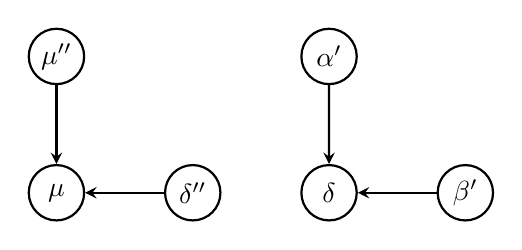
\begin{tikzpicture}[->, >=stealth, thick, scale=3.0]

    % Nodes
    \node[latent]    (mu)      {$\mu$} ; %
    \node[latent, above=of mu]    (mupp)  {$\mu''$}; %
    \node[latent, right=of mu] (deltapp) {$\delta''$};

    % More nodes
    \node[latent, right=of deltapp] (delta)  {$\delta$}; %
    \node[latent, above=of delta]  (alphap) {$\alpha'$}; %
    \node[latent, right=of delta] (betap) {$\beta'$};

    \edge {mupp} {mu}
    \edge {deltapp} {mu}
    \edge {alphap} {delta}
    \edge {betap} {delta}

\end{tikzpicture}
\end{center}

Then the joint probability of this approximate model becomes apparent:
\begin{equation}
    q(\vec{x}) = q(\mu|\mu'', \delta'')q(\delta|\alpha', \beta')
\end{equation}

So
\begin{align}
    \log{q(\vec{x})} &= \log{q(\mu|\mu'', \delta'')} + \log{q(\delta|\alpha', \beta')}
    \nonumber \\
    &= -\frac{1}{2} \log{(2\delta''\pi)} - \frac{(\mu - \mu'')^{2}}{2\delta''} +
    \alpha' \log{(\beta')} - \log{(\Gamma(\alpha'))} - (\alpha' + 1) \log{(\delta)}
    + \frac{\beta'}{\delta}
    \nonumber \\
    &= -\frac{1}{2} \log{(\delta'')} - \frac{(\mu - \mu'')^{2}}{2\delta''} +
    \alpha' \log{(\beta')} - \log{(\Gamma(\alpha'))} - (\alpha' + 1) \log{(\delta)}
    + \frac{\beta'}{\delta} + C_q
\end{align}
In this case, we are interested in $\mu, \delta, \mu'', \delta'', \alpha',
\beta'$; constants with respect to those get put in $C_q$.

\subsection{Lower Bound}

Now that we have the lower bound formula, the log joint of $p$, and the log
joint of $q$, we are ready to fully specify the lower bound formula:
\begin{align}
    L(\vec{x}, D) &= \E_{q}[\log p(\vec{x}, D)] - \E_{q}[\log q(\vec{x})]
    \nonumber \\
    &= \E_{q}[-\frac{(\mu-\mu')^{2}}{2\delta'} - (\alpha+1)\log{(\delta)} +
    \frac{\beta}{\delta} - \frac{K}{2}\log{(\delta)} -
    \frac{1}{2\delta}\sum_{k=1}^{K} (y_{k}-\mu)^{2} + C_p]
    \nonumber \\
    &\quad\quad\quad\quad - \E_{q}[-\frac{1}{2} \log{(\delta'')} - \frac{(\mu - \mu'')^{2}}{2\delta''} +
    \alpha' \log{(\beta')} - \log{(\Gamma(\alpha'))} - (\alpha' + 1) \log{(\delta)}
    + \frac{\beta'}{\delta} + C_q]
    \nonumber \\
    &= -\E_{q}[\frac{(\mu-\mu')^{2}}{2\delta'}] - \E_{q}[(\alpha+1)\log{(\delta)}] +
    \E_{q}[\frac{\beta}{\delta}] - \E_{q}[\frac{K}{2}\log{(\delta)}] -
    \E_{q}[\frac{1}{2\delta}\sum_{k=1}^{K} (y_{k}-\mu)^{2}] + \E_{q}[C_p]
    \nonumber \\
    &\quad\quad\quad\quad + \E_{q}[\frac{1}{2} \log{(\delta'')}] + \E_{q}[\frac{(\mu - \mu'')^{2}}{2\delta''}]
    \nonumber \\
    &\quad\quad\quad\quad -
    \E_{q}[\alpha' \log{(\beta')}] + \E_{q}[\log{(\Gamma(\alpha'))}] + \E_{q}[(\alpha' + 1) \log{(\delta)}]
    - \E_{q}[\frac{\beta'}{\delta}] - \E_{q}[C_q]
    \nonumber \\
    &= -\frac{1}{2\delta'}\E_{q}[(\mu-\mu')^{2}] - (\alpha+1)\E_{q}[\log{(\delta)}] +
    \beta\E_{q}[\frac{1}{\delta}] - \frac{K}{2}\E_{q}[\log{(\delta)}] -
    \frac{1}{2}\sum_{k=1}^{K}\E_{q}[\frac{(y_{k}-\mu)^{2}}{\delta}] + C_p
    \nonumber \\
    &\quad\quad\quad\quad + \frac{1}{2}\log{(\delta'')} + \frac{1}{2\delta''}\E_{q}[(\mu - \mu'')^{2}]
    \nonumber \\
    &\quad\quad\quad\quad -
    \alpha' \log{(\beta')} + \log{(\Gamma(\alpha'))} + (\alpha' + 1)\E_{q}[\log{(\delta)}]
    - \beta'\E_{q}[\frac{1}{\delta}] - C_q
    \nonumber \\
    &= -\frac{1}{2\delta'}\E_{q}[(\mu-\mu')^{2}] + (\alpha'-\alpha-\frac{K}{2})\E_{q}[\log{(\delta)}] +
    (\beta-\beta')\E_{q}[\frac{1}{\delta}] -
    \frac{1}{2}\sum_{k=1}^{K}\E_{q}[\frac{(y_{k}-\mu)^{2}}{\delta}]
    \nonumber \\
    &\quad\quad\quad\quad + \frac{1}{2}\log{(\delta'')} + \frac{1}{2\delta''}\E_{q}[(\mu - \mu'')^{2}]
    - \alpha' \log{(\beta')} + \log{(\Gamma(\alpha'))}
    + C_L
    \nonumber \\
    &= -\frac{1}{2\delta'}\E_{q}[\mu^2 -2\mu\mu' +\mu'^2] + (\alpha'-\alpha-\frac{K}{2})\E_{q}[\log{(\delta)}] +
    (\beta-\beta')\E_{q}[\frac{1}{\delta}]
    \nonumber \\
    &\quad\quad\quad\quad - \frac{1}{2}\sum_{k=1}^{K}\E_{q}[\frac{y_{k}^2 -2y_{k}\mu +\mu^{2}}{\delta}]
    \nonumber \\
    &\quad\quad\quad\quad + \frac{1}{2}\log{(\delta'')}
    + \frac{1}{2\delta''}\E_{q}[\mu^2 -2\mu\mu'' + \mu''^{2}]
    - \alpha' \log{(\beta')} + \log{(\Gamma(\alpha'))}
    + C_L
    \nonumber \\
    &= -\frac{1}{2\delta'}\E_{q}[\mu^2] +\frac{\mu'}{\delta'}\E_{q}[\mu]
    -\frac{\mu'^2}{2\delta'} + (\alpha'-\alpha-\frac{K}{2})\E_{q}[\log{(\delta)}] +
    (\beta-\beta')\E_{q}[\frac{1}{\delta}]
    \nonumber \\
    &\quad\quad\quad\quad -
    (\frac{1}{2}\sum_{k=1}^{K}y_{k}^2)\E_{q}[\frac{1}{\delta}]
    +(\sum_{k=1}^{K}y_{k})\E_{q}[\frac{\mu}{\delta}] - \frac{K}{2}\E_{q}[\frac{\mu^{2}}{\delta}]
    \nonumber \\
    &\quad\quad\quad\quad + \frac{1}{2}\log{(\delta'')}
    + \frac{1}{2\delta''}\E_{q}[\mu^2] -\frac{\mu''}{\delta''}\E_{q}[\mu] +
    \frac{\mu''^{2}}{2\delta''}
    - \alpha' \log{(\beta')} + \log{(\Gamma(\alpha'))}
    + C_L
    \nonumber \\
    &= (\frac{1}{2\delta''}-\frac{1}{2\delta'})\E_{q}[\mu^2]
    +(\frac{\mu'}{\delta'}-\frac{\mu''}{\delta''})\E_{q}[\mu]
    + (\alpha'-\alpha-\frac{K}{2})\E_{q}[\log{(\delta)}] +
    (\beta-\beta'-\sum_{k=1}^{K}\frac{y_{k}^2}{2})\E_{q}[\frac{1}{\delta}]
    \nonumber \\
    &\quad\quad\quad\quad
    +(\sum_{k=1}^{K}y_{k})\E_{q}[\frac{\mu}{\delta}] - \frac{K}{2}\E_{q}[\frac{\mu^{2}}{\delta}]
    \nonumber \\
    &\quad\quad\quad\quad + \frac{1}{2}\log{(\delta'')}
    + \frac{\mu''^{2}}{2\delta''}
    - \alpha' \log{(\beta')} + \log{(\Gamma(\alpha'))}
    + C_L
\end{align}

Let's pause here for a minute so that we can work out the expectations:

\begin{align}
    \E_{q}[\mu^2] &= \int\int \mu^2 q(\mu|\mu'',\delta'')q(\delta|\alpha', \beta')
    d\delta d\mu
    \nonumber \\
    &= \int \mu^2 q(\mu|\mu'',\delta'')\int q(\delta|\alpha', \beta')
    d\delta d\mu
    \nonumber \\
    &= \int \mu^2 q(\mu|\mu'', \delta'') d\mu
\end{align}
Note that this is the second raw moment of a normal distribution, so
\begin{align}
    \E_{q}[\mu^2] &= \int \mu^2 q(\mu|\mu'', \delta'') d\mu
    \nonumber \\
    &= \mu''^2 + \delta''^2
\end{align}
according to both \autocite{wolframNormal} (see equation 34) and
\autocite{moment2blog}.

Using a similar trick, we can see that $\E_{q}[\mu]$ is the first raw moment of
a normal distribution, so
\begin{align}
    \E_{q}[\mu] &= \mu''.
\end{align}

Now starting expectations with $\delta$,
\begin{align}
    \E_{q}[\log{\delta}] &= \int \int \log{(\delta)} q(\delta|\alpha', \beta')
    q(\mu|\mu'', \delta'') d\mu d\delta
    \nonumber \\
    &= \int \log{(\delta)} q(\delta|\alpha', \beta')
    \int q(\mu|\mu'', \delta'') d\mu d\delta
    \nonumber \\
    &= \int \log{(\delta)} q(\delta|\alpha', \beta') d\delta
\end{align}
Once again appealing to intelligent interpretation, we see that this is the
expectation of the log value for an inverse gamma distribution.  From
\autocite{invgamma}, we see that
\begin{align}
    \E_{q}[\log{\delta}] &= \log{(\beta')} - \psi(\alpha'),
\end{align}
where $\psi(\bullet)$ is the digamma function.\footnote{Although the name makes
some sense (the digamma function is the first derivative of the log gamma
function), the notation is incredibly silly, since $\psi$ is the Greek letter
\enquote{psi}.  On the other hand, the Greek letter for digamma would be
$\digamma$.  The capital $\digamma$ is F (Note that F has two horizontal strokes
(\enquote{di-}) whereas $\Gamma$ has only one).}

For the other expectation with $\delta$:
\begin{align}
    \E_{q}[\frac{1}{\delta}] &= \int \int \frac{1}{\delta} q(\delta|\alpha', \beta')
    q(\mu|\mu'', \delta'') d\mu d\delta
    \nonumber \\
    &= \int \frac{1}{\delta} q(\delta|\alpha', \beta') \int
    q(\mu|\mu'', \delta'') d\mu d\delta
    \nonumber \\
    &= \int \frac{1}{\delta} q(\delta|\alpha', \beta') d\delta
    \nonumber \\
    &= \int \frac{1}{\delta} \frac{\beta'^{\alpha'}}{\Gamma(\alpha')}
    \delta^{-\alpha' - 1} \exp{\left(\frac{-\beta'}{\delta}\right)} d\delta
    \nonumber \\
    &= \frac{\beta'^{\alpha'}}{\Gamma(\alpha')} \int \frac{1}{\delta}
    \delta^{-\alpha' - 1} \exp{\left(\frac{-\beta'}{\delta}\right)} d\delta
    \nonumber \\
    &= \frac{\beta'^{\alpha'}}{\Gamma(\alpha')} \int
    \delta^{-\alpha' - 2} \exp{\left(\frac{-\beta'}{\delta}\right)} d\delta
    \nonumber \\
    &= \frac{\beta'^{\alpha'}}{\Gamma(\alpha')} \frac{\Gamma(\alpha' -
    1)}{\beta'^{\alpha'-1}}
    \nonumber \\
    &= \frac{\beta'^{\alpha'}}{\alpha'\Gamma(\alpha'-1)} \frac{\Gamma(\alpha' -
    1)}{\beta'^{\alpha'-1}}
    \nonumber \\
    &= \frac{\beta'}{\alpha'},
\end{align}
which also happens to be given in \autocite{invgamma}.\footnote{If the
equivalence of the integral to the fraction doesn't make sense, write out the
pdf of the inverse gamma distribution, set it equal to one, pull the constants
with $\alpha$ terms out of the integral, and multiply both sides by the
reciprocal of that constant.  Now substitute $\alpha$ with
$\alpha'-1$.}\footnote{As for $\Gamma(\alpha') = \alpha'\Gamma(\alpha'-1)$,
check the definition of the gamma function.}

Now remain the expectations that deal with both $\mu$ and $\delta$.
Conveniently, we've already done the hard parts, so we substitute our findings
from the past few expectations into this part:
\begin{align}
    \E_{q}[\frac{\mu}{\delta}] &= \int \int \frac{\mu}{\delta} q(\delta|\alpha', \beta')
    q(\mu|\mu'', \delta'') d\mu d\delta
    \nonumber \\
    &= \int \int \frac{1}{\delta} q(\delta|\alpha', \beta')
    \mu q(\mu|\mu'', \delta'') d\mu d\delta
    \nonumber \\
    &= \int \frac{1}{\delta} q(\delta|\alpha', \beta')
    \int \mu q(\mu|\mu'', \delta'') d\mu d\delta
    \nonumber \\
    &= \int \frac{1}{\delta} q(\delta|\alpha', \beta')
    \mu d\delta
    \nonumber \\
    &= \mu \int \frac{1}{\delta} q(\delta|\alpha', \beta')
    d\delta
    \nonumber \\
    &= \mu'' \frac{\beta'}{\alpha'}.
\end{align}

Likewise,
\begin{align}
    \E_{q}[\frac{\mu^2}{\delta}] &= \int \int \frac{\mu^2}{\delta} q(\delta|\alpha', \beta')
    q(\mu|\mu'', \delta'') d\mu d\delta
    \nonumber \\
    &= \int \int \frac{1}{\delta} q(\delta|\alpha', \beta')
    \mu^2 q(\mu|\mu'', \delta'') d\mu d\delta
    \nonumber \\
    &= \int \frac{1}{\delta} q(\delta|\alpha', \beta')
    \int \mu^2 q(\mu|\mu'', \delta'') d\mu d\delta
    \nonumber \\
    &= \int \frac{1}{\delta} q(\delta|\alpha', \beta')
    (\mu^2 + \delta''^2) d\delta
    \nonumber \\
    &= (\mu^2 + \delta''^2) \int \frac{1}{\delta} q(\delta|\alpha', \beta')
    d\delta
    \nonumber \\
    &= (\mu''^2 + \delta''^2) \frac{\beta'}{\alpha'}.
\end{align}

Now we can substitute these expectations back into the lower bound and continue
separating terms for convenience later:
\begin{align}
    L(\vec{x}, D)
    &= (\frac{1}{2\delta''}-\frac{1}{2\delta'})\E_{q}[\mu^2]
    +(\frac{\mu'}{\delta'}-\frac{\mu''}{\delta''})\E_{q}[\mu]
    + (\alpha'-\alpha-\frac{K}{2})\E_{q}[\log{(\delta)}] +
    (\beta-\beta'-\sum_{k=1}^{K}\frac{y_{k}^2}{2})\E_{q}[\frac{1}{\delta}]
    \nonumber \\
    &\quad\quad\quad\quad
    +(\sum_{k=1}^{K}y_{k})\E_{q}[\frac{\mu}{\delta}] - \frac{K}{2}\E_{q}[\frac{\mu^{2}}{\delta}]
    \nonumber \\
    &\quad\quad\quad\quad + \frac{1}{2}\log{(\delta'')}
    + \frac{\mu''^{2}}{2\delta''}
    - \alpha' \log{(\beta')} + \log{(\Gamma(\alpha'))}
    + C_L
    \nonumber \\
    &= (\frac{1}{2\delta''}-\frac{1}{2\delta'})(\mu''^2+\delta''^2)
    +(\frac{\mu'}{\delta'}-\frac{\mu''}{\delta''})\mu''
    + (\alpha'-\alpha-\frac{K}{2})(\log(\beta')-\psi(\alpha'))
    \nonumber \\
    &\quad\quad\quad\quad
    + (\beta-\beta'-\sum_{k=1}^{K}\frac{y_{k}^2}{2})\frac{\beta'}{\alpha'}
    +(\sum_{k=1}^{K}y_{k})\frac{\beta'}{\alpha'}\mu'' -
    \frac{K\beta'}{2\alpha'}(\mu''^{2}+\delta''^2)
    \nonumber \\
    &\quad\quad\quad\quad + \frac{1}{2}\log{(\delta'')}
    + \frac{\mu''^{2}}{2\delta''}
    - \alpha' \log{(\beta')} + \log{(\Gamma(\alpha'))}
    + C_L
    \nonumber \\
    &= \frac{\mu''^2}{2\delta''}-\frac{\mu''^2}{2\delta'}
    + \frac{\delta''^2}{2\delta''}-\frac{\delta''^2}{2\delta'}
    + \frac{\mu''\mu'}{\delta'}-\frac{\mu''^2}{\delta''}
    + (\alpha'-\alpha-\frac{K}{2})\log(\beta')-(\alpha'-\alpha-\frac{K}{2})\psi(\alpha')
    \nonumber \\
    &\quad\quad\quad\quad
    + \frac{\beta\beta'}{\alpha'}-\frac{\beta'^2}{\alpha'}-\frac{\beta'}{\alpha'}\sum_{k=1}^{K}\frac{y_{k}^2}{2}
    +(\mu''\sum_{k=1}^{K}y_{k})\frac{\beta'}{\alpha'}
    - \frac{K\beta'\mu''^{2}}{2\alpha'}-\frac{K\beta'\delta''^2}{2\alpha'}
    \nonumber \\
    &\quad\quad\quad\quad + \frac{1}{2}\log{(\delta'')}
    + \frac{\mu''^{2}}{2\delta''}
    - \alpha' \log{(\beta')} + \log{(\Gamma(\alpha'))}
    + C_L
    \nonumber \\
    &= \frac{\mu''^2}{2\delta''}-\frac{\mu''^2}{2\delta'}
    + \frac{\delta''}{2}-\frac{\delta''^2}{2\delta'}
    + \frac{\mu''\mu'}{\delta'}-\frac{\mu''^2}{\delta''}
    + \frac{\mu''^{2}}{2\delta''} + \frac{1}{2}\log{(\delta'')}
    -\frac{K\beta'\delta''^2}{2\alpha'}
    - \frac{K\beta'\mu''^{2}}{2\alpha'}
    \nonumber \\
    &\quad\quad\quad\quad
    +(\mu''\sum_{k=1}^{K}y_{k})\frac{\beta'}{\alpha'}
    - (\alpha+\frac{K}{2})\log(\beta')
    + \frac{\beta\beta'}{\alpha'}-\frac{\beta'^2}{\alpha'}-\frac{\beta'}{\alpha'}\sum_{k=1}^{K}\frac{y_{k}^2}{2}
    \nonumber \\
    &\quad\quad\quad\quad
    -(\alpha'-\alpha-\frac{K}{2})\psi(\alpha')
    + \log{(\Gamma(\alpha'))}
    + C_L
    \nonumber \\
    &=
    \frac{\delta''}{2}-\frac{\delta''^2}{2\delta'}
    + \frac{\mu''\mu'}{\delta'}
    + \frac{1}{2}\log{(\delta'')}
    -\frac{K\beta'\delta''^2}{2\alpha'}
    - \frac{K\beta'\mu''^{2}}{2\alpha'}
    \nonumber \\
    &\quad\quad\quad\quad
    +(\mu''\sum_{k=1}^{K}y_{k})\frac{\beta'}{\alpha'}
    - (\alpha+\frac{K}{2})\log(\beta')
    + \frac{\beta\beta'}{\alpha'}-\frac{\beta'^2}{\alpha'}-\frac{\beta'}{\alpha'}\sum_{k=1}^{K}\frac{y_{k}^2}{2}
    \nonumber \\
    &\quad\quad\quad\quad
    -(\alpha'-\alpha-\frac{K}{2})\psi(\alpha')
    + \log{(\Gamma(\alpha'))}
    + C_L
\end{align}
This is the formulation of the lower bound we will use in the following section.
%TODO Fix E[\mu^2] (it should be \mu^2 + \delta)
%TODO Fix E[1/\delta] (it should be alpha' / beta')

\subsection{Update Rules}

Now that we know how the lower bound changes with respect to $\mu, \delta,
\mu'', \delta'', \alpha', \beta'$, we would like to know update rules to make
$\mu'', \delta'', \alpha', \beta'$ converge to their true values.  We will use
coordinate-wise ascent for finding the convergence values.  This entails taking
the derivative of the lower bound with respect to a term of interest, setting
that equal to zero, and then solving for the term of interest; this is repeated
for each term of interest.

For $\mu''$,
\begin{align}
    \frac{\partial L(\vec{x}, D)}{\partial \mu''} &=
    \frac{\mu'}{\delta'}
    - \frac{K\beta'\mu''}{\alpha'} + \frac{\beta'\sum_{k=1}^{K}y_{k}}{\alpha'}
    = 0
    \nonumber \\
    &\rightarrow
    \nonumber \\
    \frac{K\beta'\mu''}{\alpha'} &= \frac{\mu'}{\delta'}
    + \frac{\beta'\sum_{k=1}^{K}y_{k}}{\alpha'}
    \nonumber \\
    &\rightarrow
    \nonumber \\
    \mu'' &= \frac{\alpha'\mu'}{K\beta'\delta'}
    + \frac{\sum_{k=1}^{K}y_{k}}{K}
\end{align}

For $\delta''$,
\begin{align}
    \frac{\partial L(\vec{x}, D)}{\partial \delta''} &=
    \frac{1}{2} - \frac{\delta''}{\delta'}
    + \frac{1}{2\delta''} - \frac{K\beta'}{\alpha'}\delta''
    \nonumber \\
    &= -\frac{\alpha' + K\beta'\delta'}{\alpha'\delta'}\delta'' + \frac{1}{2}
    + \frac{1}{2\delta''} = 0
    \nonumber \\
    & \rightarrow
    \nonumber \\
    0 &= -\frac{2(\alpha' + K\beta'\delta')}{\alpha'\delta'}\delta''^2
    + \delta''
    + 1
    \nonumber
\end{align}
At this point, we need to use the quadratic equation:
\begin{align}
    \delta'' &= \frac{-1 \pm
    \sqrt{1 + 4\cdot\frac{2(\alpha' + K\beta'\delta')}{\alpha'\delta'}
    \cdot 1}}
    {-2\cdot\frac{2(\alpha' + K\beta'\delta')}{\alpha'\delta'}}
    \nonumber \\
    &= \frac{1 \pm
    \sqrt{1 + \frac{8(\alpha' + K\beta'\delta')}{\alpha'\delta'}}}
    {\frac{4(\alpha' + K\beta'\delta')}{\alpha'\delta'}}
    \nonumber \\
    &= \frac{\alpha'\delta' \pm
    \sqrt{(\alpha'\delta')^2 + 8(\alpha' + K\beta'\delta')(\alpha'\delta')}}
    {4(\alpha' + K\beta'\delta')}
    \nonumber \\
    &= \frac{\alpha'\delta' \pm
    \sqrt{\alpha'\delta'(\alpha'\delta' + 8(\alpha' + K\beta'\delta'))}}
    {4(\alpha' + K\beta'\delta')}
    \nonumber
\end{align}
Variance must be positive, so let's make sure of that by allowing only addition
in the numerator:
\begin{align}
    &= \frac{\alpha'\delta' +
    \sqrt{\alpha'\delta'(\alpha'\delta' + 8(\alpha' + K\beta'\delta'))}}
    {4(\alpha' + K\beta'\delta')}
\end{align}

For $\alpha'$,
\begin{align}
    \frac{\partial L(\vec{x}, D)}{\partial \alpha'} &=
    \frac{K\beta'\delta''^2}{2\alpha'^2} + \frac{K\beta'\mu''^2}{2\alpha'^2}
    - \frac{\mu''\sum_{k=1}^{K}y_{k}\beta'}{\alpha'^2}
    - \frac{\beta\beta'}{\alpha'^2} + \frac{\beta^2}{\alpha^2}
    + \frac{\beta'\sum_{1}^{K}y_{k}^2}{2\alpha'^2}
    \nonumber \\
    &\quad\quad\quad\quad
    - \psi(\alpha') - \alpha'\psi'(\alpha')
    + \alpha\psi'(\alpha') + \frac{K}{2}\psi'(\alpha')
    + \psi(\alpha')
    \nonumber \\
    &=
    \frac{K\beta'\delta''^2}{2\alpha'^2} + \frac{K\beta'\mu''^2}{2\alpha'^2}
    - \frac{2\mu''\sum_{k=1}^{K}y_{k}\beta'}{2\alpha'^2}
    - \frac{2\beta\beta'}{2\alpha'^2} + \frac{2\beta^2}{2\alpha^2}
    + \frac{\beta'\sum_{1}^{K}y_{k}^2}{2\alpha'^2}
    \nonumber \\
    &\quad\quad\quad\quad
    - \alpha'\psi'(\alpha')
    + \alpha\psi'(\alpha') + \frac{K}{2}\psi'(\alpha')
    \nonumber \\
    &\quad\quad\quad\quad
    - \psi(\alpha') - \alpha'\psi'(\alpha')
    + \alpha\psi'(\alpha') + \frac{K}{2}\psi'(\alpha')
    + \psi(\alpha')
    \nonumber \\
    &=
    \frac{K\beta'\delta''^2 + K\beta'\mu''^2
    - 2\mu''\beta'\sum_{k=1}^{K}y_{k}
    - 2\beta\beta' + 2\beta'^2
    + \beta'\sum_{k=1}^{K}y_{k}^2}{2\alpha'^2}
    \nonumber \\
    &\quad\quad\quad\quad
    + (\frac{K}{2} + \alpha - \alpha')\psi'(\alpha')
    \nonumber \\
    &=
    \frac{\beta'(K(\delta''^2 + \mu''^2)
    - 2\mu''\sum_{k=1}^{K}y_{k}
    - 2\beta + 2\beta'
    + \sum_{k=1}^{K}y_{k}^2)}{2\alpha'^2}
    \nonumber \\
    &\quad\quad\quad\quad
    + (\frac{K}{2} + \alpha - \alpha')\psi'(\alpha')
    \nonumber \\
    &=
    \beta'(K(\delta''^2 + \mu''^2)
    - 2\mu''\sum_{k=1}^{K}y_{k}
    - 2\beta + 2\beta'
    + \sum_{k=1}^{K}y_{k}^2)
    \nonumber \\
    &\quad\quad\quad\quad
    + (K\alpha'^2 + 2\alpha\alpha'^2 - 2\alpha'^3)\psi'(\alpha') = 0
    \nonumber \\
    &=
    \beta'(K(\delta''^2 + \mu''^2)
    - 2\mu''\sum_{k=1}^{K}y_{k}
    - 2\beta + 2\beta'
    + \sum_{k=1}^{K}y_{k}^2)
    \nonumber \\
    &\quad\quad\quad\quad
    + ((K + 2\alpha)\alpha'^2 - 2\alpha'^3)\psi'(\alpha') = 0
    \nonumber \\
    & \rightarrow
    \nonumber \\
    (2\alpha'^3 - (K + 2\alpha)\alpha'^2)\psi'(\alpha') &=
    \beta'(K(\delta''^2 + \mu''^2)
    - 2\mu''\sum_{k=1}^{K}y_{k}
    - 2\beta + 2\beta'
    + \sum_{k=1}^{K}y_{k}^2)
\end{align}
Hmm...I have no idea how to solve for $\alpha'$ at this point.

For $\beta'$,
\begin{align}
    \frac{\partial L(\vec{x}, D)}{\partial \beta'} &=
    - \frac{K\delta''^2}{2\alpha'} - \frac{K\mu''^2}{2\alpha'}
    + \frac{\mu''\sum_{k=1}^{K}y_{k}}{\alpha'}
    - \frac{\alpha + \frac{K}{2}}{\beta'}
    + \frac{\beta}{\alpha'} - \frac{2}{\alpha'}\beta'
    - \frac{\sum_{k=1}^{K} y_{k}^2}{2\alpha'}
    \nonumber \\
    &= \frac{2\beta + 2\mu''\sum_{k=1}^{K}y_{k}
    - K\delta''^2 - K\mu''^2
    - \sum_{k=1}^{K} y_{k}^2}{2\alpha'}
    - \frac{\alpha + \frac{K}{2}}{\beta'}
    - \frac{2}{\alpha'}\beta'
    \nonumber \\
    &=
    - \frac{2}{\alpha'}\beta'^2
    + \frac{2\beta + 2\mu''\sum_{k=1}^{K}y_{k}
    - K\delta''^2 - K\mu''^2
    - \sum_{k=1}^{K} y_{k}^2}{2\alpha'}\beta'
    - (\alpha + \frac{K}{2})
    \nonumber \\
    &=
    - \frac{2}{\alpha'}\beta'^2
    + \frac{2\beta + 2\mu''\sum_{k=1}^{K}y_{k}
    - K(\delta''^2 + \mu''^2)
    - \sum_{k=1}^{K} y_{k}^2}{2\alpha'}\beta'
    - (\alpha + \frac{K}{2})
    \nonumber
\end{align}
Again, we need to use the quadratic equation:
\begin{align}
    \beta' &= \frac{- \frac{2\beta + 2\mu''\sum_{k=1}^{K}y_{k} - K(\delta''^2 +
    \mu''^2) - \sum_{k=1}^{K} y_{k}^{2}}{2\alpha'}}{-\frac{4}{\alpha'}}
    \nonumber \\
    &\quad\quad\quad\quad
    \pm
    \frac{\sqrt{\frac{1}{4\alpha'^2}(2\beta + 2\mu''\sum_{k=1}^{K}y_{k} - K(\delta''^2 +
    \mu''^2) - \sum_{k=1}^{K} y_{k}^{2})^2 - \frac{8}{\alpha'}(\alpha +
    \frac{K}{2})}}
    {-\frac{4}{\alpha'}}
    \nonumber \\
    &= \frac{2\beta + 2\mu''\sum_{k=1}^{K}y_{k} - K(\delta''^2 +
    \mu''^2) - \sum_{k=1}^{K} y_{k}^{2}}{8}
    \nonumber \\
    &\quad\quad\quad\quad
    \pm
    \sqrt{\frac{1}{64}(2\beta + 2\mu''\sum_{k=1}^{K}y_{k} - K(\delta''^2 +
    \mu''^2) - \sum_{k=1}^{K} y_{k}^{2})^2 - \frac{1}{2}\alpha'(\alpha +
    \frac{K}{2})}
    \nonumber
\end{align}
Here also we know that $\beta' > 0$, so we choose to permit addition only:
\begin{align}
    \beta' &= \frac{2\beta + 2\mu''\sum_{k=1}^{K}y_{k} - K(\delta''^2 +
    \mu''^2) - \sum_{k=1}^{K} y_{k}^{2}}{8}
    \nonumber \\
    &\quad\quad\quad\quad
    +
    \sqrt{\frac{1}{64}(2\beta + 2\mu''\sum_{k=1}^{K}y_{k} - K(\delta''^2 +
    \mu''^2) - \sum_{k=1}^{K} y_{k}^{2})^2 - \frac{1}{2}\alpha'(\alpha +
    \frac{K}{2})}
    \nonumber
\end{align}
\end{appendices}
\fi

\printbibliography

\end{document}
